\PassOptionsToPackage{unicode=true}{hyperref} % options for packages loaded elsewhere
\PassOptionsToPackage{hyphens}{url}
%
\documentclass[]{article}
\usepackage{lmodern}
\usepackage{amssymb,amsmath}
\usepackage{ifxetex,ifluatex}
\usepackage{fixltx2e} % provides \textsubscript
\ifnum 0\ifxetex 1\fi\ifluatex 1\fi=0 % if pdftex
  \usepackage[T1]{fontenc}
  \usepackage[utf8]{inputenc}
  \usepackage{textcomp} % provides euro and other symbols
\else % if luatex or xelatex
  \usepackage{unicode-math}
  \defaultfontfeatures{Ligatures=TeX,Scale=MatchLowercase}
\fi
% use upquote if available, for straight quotes in verbatim environments
\IfFileExists{upquote.sty}{\usepackage{upquote}}{}
% use microtype if available
\IfFileExists{microtype.sty}{%
\usepackage[]{microtype}
\UseMicrotypeSet[protrusion]{basicmath} % disable protrusion for tt fonts
}{}
\IfFileExists{parskip.sty}{%
\usepackage{parskip}
}{% else
\setlength{\parindent}{0pt}
\setlength{\parskip}{6pt plus 2pt minus 1pt}
}
\usepackage{hyperref}
\hypersetup{
            pdftitle={Sample homework},
            pdfauthor={Bob Settlage},
            pdfborder={0 0 0},
            breaklinks=true}
\urlstyle{same}  % don't use monospace font for urls
\usepackage[margin=1in]{geometry}
\usepackage{color}
\usepackage{fancyvrb}
\newcommand{\VerbBar}{|}
\newcommand{\VERB}{\Verb[commandchars=\\\{\}]}
\DefineVerbatimEnvironment{Highlighting}{Verbatim}{commandchars=\\\{\}}
% Add ',fontsize=\small' for more characters per line
\usepackage{framed}
\definecolor{shadecolor}{RGB}{248,248,248}
\newenvironment{Shaded}{\begin{snugshade}}{\end{snugshade}}
\newcommand{\AlertTok}[1]{\textcolor[rgb]{0.94,0.16,0.16}{#1}}
\newcommand{\AnnotationTok}[1]{\textcolor[rgb]{0.56,0.35,0.01}{\textbf{\textit{#1}}}}
\newcommand{\AttributeTok}[1]{\textcolor[rgb]{0.77,0.63,0.00}{#1}}
\newcommand{\BaseNTok}[1]{\textcolor[rgb]{0.00,0.00,0.81}{#1}}
\newcommand{\BuiltInTok}[1]{#1}
\newcommand{\CharTok}[1]{\textcolor[rgb]{0.31,0.60,0.02}{#1}}
\newcommand{\CommentTok}[1]{\textcolor[rgb]{0.56,0.35,0.01}{\textit{#1}}}
\newcommand{\CommentVarTok}[1]{\textcolor[rgb]{0.56,0.35,0.01}{\textbf{\textit{#1}}}}
\newcommand{\ConstantTok}[1]{\textcolor[rgb]{0.00,0.00,0.00}{#1}}
\newcommand{\ControlFlowTok}[1]{\textcolor[rgb]{0.13,0.29,0.53}{\textbf{#1}}}
\newcommand{\DataTypeTok}[1]{\textcolor[rgb]{0.13,0.29,0.53}{#1}}
\newcommand{\DecValTok}[1]{\textcolor[rgb]{0.00,0.00,0.81}{#1}}
\newcommand{\DocumentationTok}[1]{\textcolor[rgb]{0.56,0.35,0.01}{\textbf{\textit{#1}}}}
\newcommand{\ErrorTok}[1]{\textcolor[rgb]{0.64,0.00,0.00}{\textbf{#1}}}
\newcommand{\ExtensionTok}[1]{#1}
\newcommand{\FloatTok}[1]{\textcolor[rgb]{0.00,0.00,0.81}{#1}}
\newcommand{\FunctionTok}[1]{\textcolor[rgb]{0.00,0.00,0.00}{#1}}
\newcommand{\ImportTok}[1]{#1}
\newcommand{\InformationTok}[1]{\textcolor[rgb]{0.56,0.35,0.01}{\textbf{\textit{#1}}}}
\newcommand{\KeywordTok}[1]{\textcolor[rgb]{0.13,0.29,0.53}{\textbf{#1}}}
\newcommand{\NormalTok}[1]{#1}
\newcommand{\OperatorTok}[1]{\textcolor[rgb]{0.81,0.36,0.00}{\textbf{#1}}}
\newcommand{\OtherTok}[1]{\textcolor[rgb]{0.56,0.35,0.01}{#1}}
\newcommand{\PreprocessorTok}[1]{\textcolor[rgb]{0.56,0.35,0.01}{\textit{#1}}}
\newcommand{\RegionMarkerTok}[1]{#1}
\newcommand{\SpecialCharTok}[1]{\textcolor[rgb]{0.00,0.00,0.00}{#1}}
\newcommand{\SpecialStringTok}[1]{\textcolor[rgb]{0.31,0.60,0.02}{#1}}
\newcommand{\StringTok}[1]{\textcolor[rgb]{0.31,0.60,0.02}{#1}}
\newcommand{\VariableTok}[1]{\textcolor[rgb]{0.00,0.00,0.00}{#1}}
\newcommand{\VerbatimStringTok}[1]{\textcolor[rgb]{0.31,0.60,0.02}{#1}}
\newcommand{\WarningTok}[1]{\textcolor[rgb]{0.56,0.35,0.01}{\textbf{\textit{#1}}}}
\usepackage{longtable,booktabs}
% Fix footnotes in tables (requires footnote package)
\IfFileExists{footnote.sty}{\usepackage{footnote}\makesavenoteenv{longtable}}{}
\usepackage{graphicx,grffile}
\makeatletter
\def\maxwidth{\ifdim\Gin@nat@width>\linewidth\linewidth\else\Gin@nat@width\fi}
\def\maxheight{\ifdim\Gin@nat@height>\textheight\textheight\else\Gin@nat@height\fi}
\makeatother
% Scale images if necessary, so that they will not overflow the page
% margins by default, and it is still possible to overwrite the defaults
% using explicit options in \includegraphics[width, height, ...]{}
\setkeys{Gin}{width=\maxwidth,height=\maxheight,keepaspectratio}
\setlength{\emergencystretch}{3em}  % prevent overfull lines
\providecommand{\tightlist}{%
  \setlength{\itemsep}{0pt}\setlength{\parskip}{0pt}}
\setcounter{secnumdepth}{0}
% Redefines (sub)paragraphs to behave more like sections
\ifx\paragraph\undefined\else
\let\oldparagraph\paragraph
\renewcommand{\paragraph}[1]{\oldparagraph{#1}\mbox{}}
\fi
\ifx\subparagraph\undefined\else
\let\oldsubparagraph\subparagraph
\renewcommand{\subparagraph}[1]{\oldsubparagraph{#1}\mbox{}}
\fi

% set default figure placement to htbp
\makeatletter
\def\fps@figure{htbp}
\makeatother


\title{Sample homework}
\author{Bob Settlage}
\date{2019-07-12}

\begin{document}
\maketitle

This is a sample of how I would like the homework to look when turned
in. This is a sample of how I would like the homework to look when
turned in. \emph{It will look a bit better imo, because you will knit to
pdf rather than html as shown here.}

\hypertarget{homework-1}{%
\section{Homework 1}\label{homework-1}}

\hypertarget{your-name}{%
\section{Your Name}\label{your-name}}

\hypertarget{date}{%
\section{Date}\label{date}}

\hypertarget{problem-1}{%
\subsection{Problem 1}\label{problem-1}}

This is an R Markdown document. Markdown is a simple formatting syntax
for authoring HTML, PDF, and MS Word documents. For more details on
using R Markdown see \url{http://rmarkdown.rstudio.com}.

You can embed an R code chunk like this, note that \texttt{kable} makes
REALLY nice tables with ZERO effort as seen in Table 1. Don't just print
output to consol, use kable!! In my opinion, including code to create
tables in-line is a detraction, this is simple to show you how easy it
is to do it. Code that is relevant to the problem should be included,
code that is for display or as a summary, should be omitted in-line and
it is up to you on if it should be included in an Appendix.

\begin{Shaded}
\begin{Highlighting}[]
\CommentTok{##### }
\CommentTok{##### }
\CommentTok{##### Problem 1: Data summary #####}
\CommentTok{##### output using kable}
\CommentTok{##### }
\CommentTok{##### }
\NormalTok{knitr}\OperatorTok{::}\KeywordTok{kable}\NormalTok{(}\KeywordTok{summary}\NormalTok{(cars), }\DataTypeTok{caption =} \StringTok{"Quick summary of car data."}\NormalTok{)}
\end{Highlighting}
\end{Shaded}

\begin{longtable}[]{@{}lll@{}}
\caption{Quick summary of car data.}\tabularnewline
\toprule
& speed & dist\tabularnewline
\midrule
\endfirsthead
\toprule
& speed & dist\tabularnewline
\midrule
\endhead
& Min. : 4.0 & Min. : 2.00\tabularnewline
& 1st Qu.:12.0 & 1st Qu.: 26.00\tabularnewline
& Median :15.0 & Median : 36.00\tabularnewline
& Mean :15.4 & Mean : 42.98\tabularnewline
& 3rd Qu.:19.0 & 3rd Qu.: 56.00\tabularnewline
& Max. :25.0 & Max. :120.00\tabularnewline
\bottomrule
\end{longtable}

Likewise, \texttt{stargazer} simplifies making tables of linear model
output. See Table 2 below. See how simple?? Note that you don't need to
set the type AND it will look better when knit to pdf.

\begin{Shaded}
\begin{Highlighting}[]
\CommentTok{##### }
\CommentTok{##### }
\CommentTok{##### Problem 1: Quick lm #####}
\CommentTok{##### output using Stargazer}
\CommentTok{##### }
\CommentTok{##### }
\NormalTok{fit <-}\StringTok{ }\KeywordTok{lm}\NormalTok{(dist }\OperatorTok{~}\StringTok{ }\NormalTok{speed, }\DataTypeTok{data =}\NormalTok{ cars)}
\KeywordTok{stargazer}\NormalTok{(fit,}\DataTypeTok{header =}\NormalTok{ F,}\DataTypeTok{type =} \StringTok{"html"}\NormalTok{) }
\end{Highlighting}
\end{Shaded}

Dependent variable:

dist

speed

3.932***

(0.416)

Constant

-17.579**

(6.758)

Observations

50

R2

0.651

Adjusted R2

0.644

Residual Std. Error

15.380 (df = 48)

F Statistic

89.567*** (df = 1; 48)

Note:

\emph{p\textless{}0.1; \textbf{p\textless{}0.05; }}p\textless{}0.01

\hypertarget{problem-2}{%
\subsection{Problem 2}\label{problem-2}}

You can also embed plots and have Rmarkdown figure out the figure number
automatically. Make sure and name the code chuck and then reference the
figure using \texttt{\textbackslash{}@ref(fig:Problem2a)}. See Figure
@ref(fig:Problem2a) for example (note, this shows up correctly when knit
to pdf):

\begin{Shaded}
\begin{Highlighting}[]
\CommentTok{##### }
\CommentTok{##### }
\CommentTok{##### Problem 2: plot #####}
\CommentTok{##### making a pie chart}
\CommentTok{##### }
\CommentTok{##### }
\KeywordTok{par}\NormalTok{(}\DataTypeTok{mar =} \KeywordTok{c}\NormalTok{(}\DecValTok{0}\NormalTok{, }\DecValTok{1}\NormalTok{, }\DecValTok{0}\NormalTok{, }\DecValTok{1}\NormalTok{))}
\KeywordTok{pie}\NormalTok{(}
  \KeywordTok{c}\NormalTok{(}\DecValTok{280}\NormalTok{, }\DecValTok{60}\NormalTok{, }\DecValTok{20}\NormalTok{),}
  \KeywordTok{c}\NormalTok{(}\StringTok{'Sky'}\NormalTok{, }\StringTok{'Sunny side of pyramid'}\NormalTok{, }\StringTok{'Shady side of pyramid'}\NormalTok{),}
  \DataTypeTok{col =} \KeywordTok{c}\NormalTok{(}\StringTok{'#0292D8'}\NormalTok{, }\StringTok{'#F7EA39'}\NormalTok{, }\StringTok{'#C4B632'}\NormalTok{),}
  \DataTypeTok{init.angle =} \DecValTok{-50}\NormalTok{, }\DataTypeTok{border =} \OtherTok{NA}
\NormalTok{)}
\end{Highlighting}
\end{Shaded}

\begin{figure}
\centering
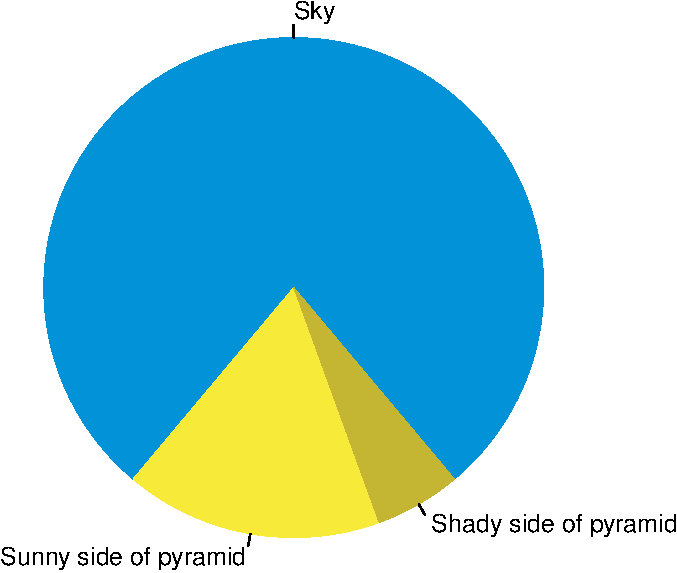
\includegraphics{SampleHomework_files/figure-latex/Problem2a-1.pdf}
\caption{A fancy pie chart.}
\end{figure}

\begin{center}\rule{0.5\linewidth}{0.5pt}\end{center}

\hypertarget{appendix-1-r-code}{%
\section{Appendix 1: R code}\label{appendix-1-r-code}}

If you name the code chucks, it is easy to include code not really
important to the main text but necessary as an Appendix. For instance:

\begin{Shaded}
\begin{Highlighting}[]
\CommentTok{##### }
\CommentTok{##### }
\CommentTok{##### Project setup #####}
\CommentTok{##### }
\CommentTok{##### }
\CommentTok{##### }
\NormalTok{knitr}\OperatorTok{::}\NormalTok{opts_chunk}\OperatorTok{$}\KeywordTok{set}\NormalTok{(}\DataTypeTok{collapse =} \OtherTok{TRUE}\NormalTok{)}
\KeywordTok{library}\NormalTok{(stargazer)}
\CommentTok{##### }
\CommentTok{##### }
\CommentTok{##### }
\CommentTok{##### }
\CommentTok{##### Problem 1: Data summary #####}
\CommentTok{##### output using kable}
\CommentTok{##### }
\CommentTok{##### }
\NormalTok{knitr}\OperatorTok{::}\KeywordTok{kable}\NormalTok{(}\KeywordTok{summary}\NormalTok{(cars), }\DataTypeTok{caption =} \StringTok{"Quick summary of car data."}\NormalTok{)}
\CommentTok{##### }
\CommentTok{##### }
\CommentTok{##### Problem 1: Quick lm #####}
\CommentTok{##### output using Stargazer}
\CommentTok{##### }
\CommentTok{##### }
\NormalTok{fit <-}\StringTok{ }\KeywordTok{lm}\NormalTok{(dist }\OperatorTok{~}\StringTok{ }\NormalTok{speed, }\DataTypeTok{data =}\NormalTok{ cars)}
\KeywordTok{stargazer}\NormalTok{(fit,}\DataTypeTok{header =}\NormalTok{ F,}\DataTypeTok{type =} \StringTok{"html"}\NormalTok{) }
\CommentTok{##### }
\CommentTok{##### }
\CommentTok{##### Problem 2: plot #####}
\CommentTok{##### making a pie chart}
\CommentTok{##### }
\CommentTok{##### }
\KeywordTok{par}\NormalTok{(}\DataTypeTok{mar =} \KeywordTok{c}\NormalTok{(}\DecValTok{0}\NormalTok{, }\DecValTok{1}\NormalTok{, }\DecValTok{0}\NormalTok{, }\DecValTok{1}\NormalTok{))}
\KeywordTok{pie}\NormalTok{(}
  \KeywordTok{c}\NormalTok{(}\DecValTok{280}\NormalTok{, }\DecValTok{60}\NormalTok{, }\DecValTok{20}\NormalTok{),}
  \KeywordTok{c}\NormalTok{(}\StringTok{'Sky'}\NormalTok{, }\StringTok{'Sunny side of pyramid'}\NormalTok{, }\StringTok{'Shady side of pyramid'}\NormalTok{),}
  \DataTypeTok{col =} \KeywordTok{c}\NormalTok{(}\StringTok{'#0292D8'}\NormalTok{, }\StringTok{'#F7EA39'}\NormalTok{, }\StringTok{'#C4B632'}\NormalTok{),}
  \DataTypeTok{init.angle =} \DecValTok{-50}\NormalTok{, }\DataTypeTok{border =} \OtherTok{NA}
\NormalTok{)}
\end{Highlighting}
\end{Shaded}

\end{document}
